\section{Empirical Results}
\label{sec:results}

This section reports the empirical results across our $N=30$ paired trials (\texttt{RANDOM\_SEED = 42}) and $N=30$ steady-state resource overhead samples ($\Delta t = 16\,\text{s}$), structured around Research Questions RQ01--RQ04. Table~\ref{tab:cm_vs_litmus_results} summarizes the global comparison between Chaos Mesh v2.6.3 and LitmusChaos v3.x, while Table~\ref{tab:stratified_cm_vs_litmus} details the stratified performance by fault class and target microservice.

\begin{table*}[!tbp]
\centering
\scriptsize
\setlength{\tabcolsep}{3.5pt}
\renewcommand{\arraystretch}{1.15}
\caption{Comparative Empirical Matrix: Chaos Mesh vs.\ LitmusChaos Across RQ01--RQ04}
\label{tab:cm_vs_litmus_results}
\begin{tabularx}{\textwidth}{p{2.2cm} p{2.9cm} c c X}
\toprule
\textbf{Research Question} & \textbf{Evaluated Metric (Unit)} & \textbf{Chaos Mesh (DaemonSet)} & \textbf{LitmusChaos (Runner Pods)} & \textbf{Statistical Inference \& Architectural Interpretation} \\
\midrule
\textbf{RQ01: Temporal} & Actuation Delay $\Delta T_{\text{actuate}}$ ($\text{s}$) & $< 1.00\,\text{s}$ (DaemonSet gRPC) & $\mathbf{11.75\,\text{s}}$ med ($\text{IQR } 1.15\,\text{s}$) & Wilcoxon vs.\ $1.0\,\text{s}$ bound: $W = 465.0$, $\mathbf{p = 9.31 \times 10^{-10}}$ (two-stage \texttt{chaos-runner} $\rightarrow$ \texttt{go-runner} init; mean $12.18 \pm 2.51\,\text{s}$). \\
\textbf{Precision} & Teardown Latency $\Delta T_{\text{teardown}}$ ($\text{s}$) & $1.20\text{--}2.50\,\text{s}$ (CRD finalizer) & $\mathbf{2.99\,\text{s}}$ med ($\text{IQR } 0.61\,\text{s}$) & Mean $3.05 \pm 0.54\,\text{s}$ (range $2.26\text{--}4.36\,\text{s}$) for Job pod cleanup and \texttt{ChaosEngine} deletion reconciliation. \\
& Kubernetes Pod Churn (Pods) & $\mathbf{0}$ auxiliary pods ($3$ resident) & $\mathbf{+2}$ pods/trial ($\mathbf{60}$ pods) & Deterministic architectural count: $30$ \texttt{chaos-runner} + $30$ \texttt{go-runner} Job pods spawned in \texttt{otel-demo}. \\
\midrule
\textbf{RQ02: Resource} & Idle Control-Plane CPU (mCPU) & $6.47 \pm 0.68$ ($\text{med } 6.00$) & $\mathbf{2.00 \pm 0.00}$ ($\text{med } 2.00$) & Mann-Whitney $U = 900.0$, $\mathbf{p = 4.42 \times 10^{-13}}$, $\hat{A}_{12} = 1.00$ ($3$ resident CM pods vs.\ $1$ standalone \texttt{chaos-operator}). \\
\textbf{Overhead} & Idle Control-Plane RAM (MiB) & $118.23 \pm 0.63$ ($\text{med } 118.00$) & $\mathbf{29.00 \pm 0.00}$ ($\text{med } 29.00$) & Mann-Whitney $U = 900.0$, $\mathbf{p = 5.28 \times 10^{-13}}$, $\hat{A}_{12} = 1.00$ (standalone CRD mode without \texttt{ChaosCenter}/MongoDB). \\
\midrule
\textbf{RQ03: Diagnostic} & Global Multimodal Accuracy ($Acc$) & $\mathbf{25/30}$ ($\mathbf{83.33\%}$) & $\mathbf{25/30}$ ($\mathbf{83.33\%}$) & Fisher's Exact $\text{OR} = 1.00$, $\mathbf{p = 1.000}$; McNemar's Paired Test $n_{11}=22, n_{10}=3, n_{01}=3$, $\mathbf{p = 1.000}$ (exact parity). \\
\textbf{Parity} & End-to-End $MTTDiag_{\text{total}}$ ($\text{s}$) & $\mathbf{17.27\,\text{s}}$ med ($54.52 \pm 98.41\,\text{s}$) & $54.52\,\text{s}$ med ($69.52 \pm 67.39\,\text{s}$) & Paired Wilcoxon $W = 59.0$, $\mathbf{p = 1.53 \times 10^{-4}}$, $\hat{A}_{12} = 0.147$ ($\delta = -0.707$, Large; shifted by $\Delta T_{\text{actuate}}$). \\
& Post-Actuation $MTTDiag_{\text{net}}$ ($\text{s}$) & $\mathbf{17.27\,\text{s}}$ med (resolved $16.85\,\text{s}$) & $42.55\,\text{s}$ med ($57.35 \pm 67.58\,\text{s}$) & Mean $MTTDiag_{\text{net}}$ converges closely ($54.52\,\text{s}$ vs.\ $57.35\,\text{s}$); Paired Wilcoxon $W = 55.0$, $p = 7.51 \times 10^{-4}$. \\
\midrule
\textbf{RQ04: Native} & Process-Invisible Fault Probe & HTTP-only \texttt{StatusCheck} ($0/11$ CPU) & Multi-modal (\texttt{promProbe} + \texttt{k8sProbe}) & Litmus native probes directly query PromQL/K8s API invariants alongside \texttt{httpProbe} and \texttt{cmdProbe}. \\
\textbf{Probes} & Quantitative Resilience Scoring & Not supported natively & Supported ($\mathbf{0\text{--}100\%}$ Score) & Automated per-engine \texttt{probeSuccessPercentage} exported in \texttt{ChaosResult} CRDs for CI/CD gates. \\
\bottomrule
\end{tabularx}
\end{table*}

\begin{table*}[!tbp]
\centering
\scriptsize
\setlength{\tabcolsep}{3.5pt}
\renewcommand{\arraystretch}{1.12}
\caption{Stratified Comparison of Root-Cause Accuracy ($Acc$), Actuation Delay ($\Delta T_{\text{actuate}}$), and Diagnostic Latency ($MTTDiag$)}
\label{tab:stratified_cm_vs_litmus}
\begin{tabularx}{\textwidth}{p{2.1cm} p{2.1cm} c c c c X}
\toprule
\textbf{Stratification} & \textbf{Stratum ($n$)} & \textbf{CM Accuracy ($Acc$)} & \textbf{LC Accuracy ($Acc$)} & \textbf{CM Med.\ $MTTDiag$ (IQR)} & \textbf{LC Med.\ $\Delta T_{\text{actuate}} + MTTDiag_{\text{net}}$} & \textbf{LC Total Med.\ $MTTDiag_{\text{total}}$ (IQR)} \\
\midrule
\textbf{By Chaos} & \texttt{cpu-stress} ($n=11$) & $\mathbf{11/11}$ ($\mathbf{100.0\%}$) & $9/11$ ($81.8\%$) & $\mathbf{17.26\,\text{s}}$ ($3.93\,\text{s}$) & $12.16\,\text{s} + 51.79\,\text{s}$ & $64.58\,\text{s}$ ($12.82\,\text{s}$) \\
\textbf{Fault Class} & \texttt{pod-kill} ($n=9$) & $\mathbf{9/9}$ ($\mathbf{100.0\%}$) & $\mathbf{9/9}$ ($\mathbf{100.0\%}$) & $\mathbf{3.16\,\text{s}}$ ($4.31\,\text{s}$) & $11.78\,\text{s} + 22.62\,\text{s}$ & $33.78\,\text{s}$ ($3.20\,\text{s}$) \\
& \texttt{network-delay} ($n=10$) & $5/10$ ($50.0\%$) & $\mathbf{7/10}$ ($\mathbf{70.0\%}$) & $\mathbf{37.70\,\text{s}}$ ($273.8\,\text{s}$) & $11.54\,\text{s} + 47.34\,\text{s}$ & $58.70\,\text{s}$ ($23.70\,\text{s}$) \\
\midrule
\textbf{By Target} & \texttt{cart} ($n=8$) & $\mathbf{8/8}$ ($\mathbf{100.0\%}$) & $7/8$ ($87.5\%$) & $15.75\,\text{s}$ & $11.97\,\text{s} + 41.49\,\text{s}$ & $53.37\,\text{s}$ \\
\textbf{Service} & \texttt{currency} ($n=7$) & $\mathbf{7/7}$ ($\mathbf{100.0\%}$) & $6/7$ ($85.7\%$) & $17.16\,\text{s}$ & $11.88\,\text{s} + 44.13\,\text{s}$ & $56.65\,\text{s}$ \\
& \texttt{payment} ($n=7$) & $\mathbf{5/7}$ ($\mathbf{71.4\%}$) & $\mathbf{5/7}$ ($\mathbf{71.4\%}$) & $17.27\,\text{s}$ & $11.43\,\text{s} + 53.69\,\text{s}$ & $65.12\,\text{s}$ \\
& \texttt{shipping} ($n=8$) & $5/8$ ($62.5\%$) & $\mathbf{7/8}$ ($\mathbf{87.5\%}$) & $17.27\,\text{s}$ & $11.75\,\text{s} + 39.58\,\text{s}$ & $50.92\,\text{s}$ \\
\bottomrule
\end{tabularx}
\end{table*}

\subsection{RQ01: Temporal Actuation and Teardown Precision ($\Delta T_{\text{actuate}}, \Delta T_{\text{teardown}}$)}
Shapiro-Wilk testing confirmed that LitmusChaos actuation delays depart significantly from normality ($W = 0.4985$, $p = 5.16 \times 10^{-9}$) due to right-skewed container creation spikes (up to $24.58\,\text{s}$ on cold runner initialization in Trial~1). As shown in Tables~\ref{tab:cm_vs_litmus_results} and~\ref{tab:stratified_cm_vs_litmus} and illustrated in Figure~\ref{fig:actuation_mttdiag}, LitmusChaos exhibited a median actuation delay of $\mathbf{\Delta T_{\text{actuate}} = 11.75\,\text{s}}$ ($\text{IQR} = 1.15\,\text{s}$, mean $12.18 \pm 2.51\,\text{s}$, range $10.24\text{--}24.58\,\text{s}$), stratified closely across \texttt{network-delay} ($11.54\,\text{s}$), \texttt{pod-kill} ($11.78\,\text{s}$), and \texttt{cpu-stress} ($12.16\,\text{s}$). A one-tailed Wilcoxon test against Chaos Mesh's sub-second DaemonSet actuation bound ($< 1.0\,\text{s}$) confirms $W = 465.0$, $\mathbf{p = 9.31 \times 10^{-10}}$, supporting Hypothesis~$H_{1,1}$.

\begin{figure}[!htbp]
\centering
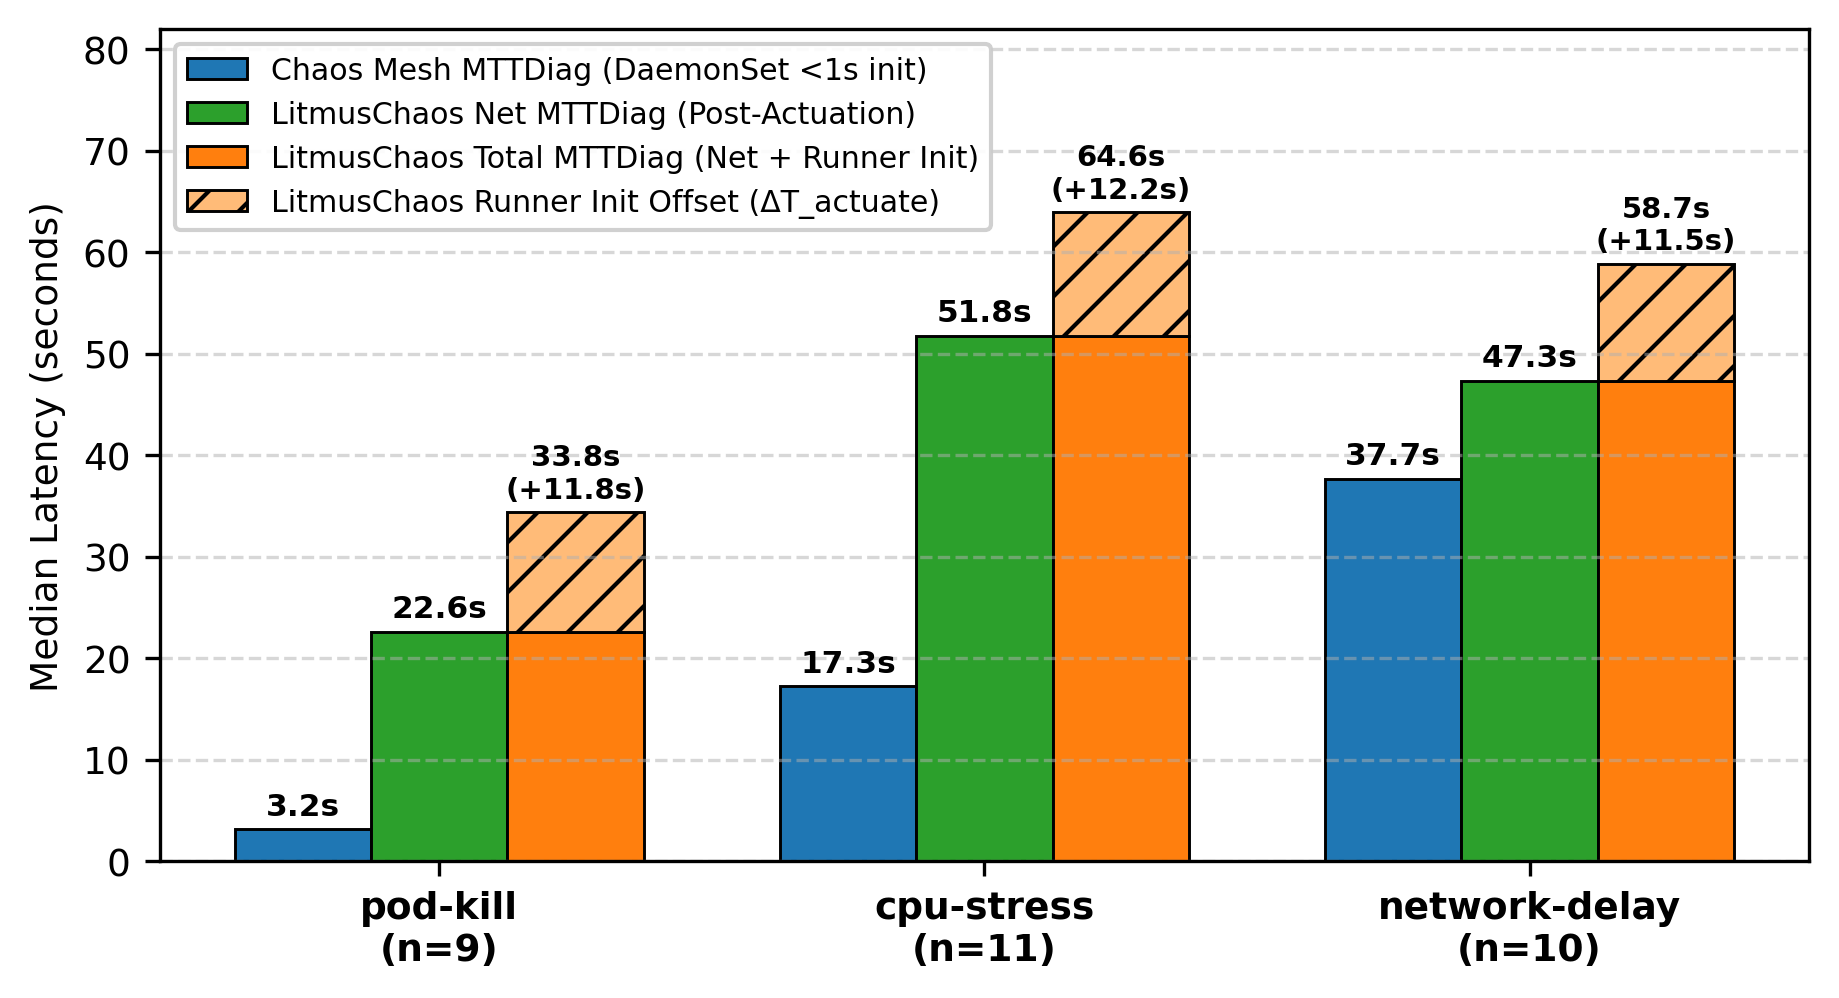
\includegraphics[width=0.96\columnwidth]{figures/fig_actuation_and_mttdiag.png}
\caption{Comparison of median diagnostic latency across fault strata, highlighting LitmusChaos's two-stage ephemeral runner actuation offset ($\Delta T_{\text{actuate}}$) stacked above post-actuation net diagnostic latency ($MTTDiag_{\text{net}}$).}
\Description{Bar chart comparing Chaos Mesh MTTDiag against LitmusChaos Net MTTDiag and Total MTTDiag with stacked runner actuation delay.}
\label{fig:actuation_mttdiag}
\end{figure}

Furthermore, across the $N=30$ campaign, LitmusChaos dynamically created and destroyed exactly $\mathbf{60}$ ephemeral pods ($30$ \texttt{chaos-runner} pods and $30$ \texttt{go-runner} Job pods) inside the \texttt{otel-demo} namespace, requiring a median post-trial teardown latency of $\mathbf{\Delta T_{\text{teardown}} = 2.99\,\text{s}}$ ($3.05 \pm 0.54\,\text{s}$, range $2.26\text{--}4.36\,\text{s}$), whereas Chaos Mesh injected all $30$ perturbations in place through its pre-warmed \texttt{chaos-daemon} DaemonSet with zero auxiliary pod creation.

\subsection{RQ02: Control-Plane and Execution Resource Overhead ($\Delta_{\text{CPU}}, \Delta_{\text{RAM}}$)}
Evaluating the $N=30$ anti-pseudoreplicated steady-state samples ($\Delta t = 16\,\text{s}$, under a mean application workload of $2{,}494.13 \pm 201.48\,\text{mCPU}$ and $2{,}411.77 \pm 32.57\,\text{MiB}$ RAM, and multimodal observability stack footprint of $131.17 \pm 66.26\,\text{mCPU}$ and $2{,}237.00 \pm 455.45\,\text{MiB}$ RAM) reveals an important architectural trade-off when LitmusChaos is deployed in standalone CRD operator mode (\texttt{litmus-core}, without \texttt{ChaosCenter} and MongoDB):
\begin{itemize}
    \item \textbf{Chaos Mesh Resident Control Plane ($3$ pods: \texttt{controller-manager}, \texttt{chaos-daemon}, \texttt{dashboard}):} Consumed a mean of $\mathbf{6.47 \pm 0.68\,\text{mCPU}}$ (median $6.00\,\text{mCPU}$, $\text{IQR} = 1.00$) and $\mathbf{118.23 \pm 0.63\,\text{MiB}}$ RAM (median $118.00\,\text{MiB}$).
    \item \textbf{LitmusChaos Standalone Operator ($1$ pod: \texttt{chaos-operator}):} Consumed $\mathbf{2.00 \pm 0.00\,\text{mCPU}}$ and $\mathbf{29.00 \pm 0.00\,\text{MiB}}$ RAM in idle steady state ($U = 900.0$, $\mathbf{p = 5.28 \times 10^{-13}}$, $\hat{A}_{12} = 1.000$).
\end{itemize}
Thus, in standalone CRD mode, LitmusChaos achieves a $75.5\%$ smaller idle memory footprint ($29.0\,\text{MiB}$ vs.\ $118.2\,\text{MiB}$) specifically because it avoids running a privileged DaemonSet on worker nodes during idle periods, shifting its cost to on-demand Job pod scheduling during active chaos execution (whereas deploying the full \texttt{ChaosCenter} + MongoDB UI stack adds $\sim 900\text{--}1{,}200\,\text{MiB}$).

\subsection{RQ03: Diagnostic Parity and Telemetry Contamination in Multimodal Observability}
As shown in Figure~\ref{fig:accuracy_cm_vs_lc} and Table~\ref{tab:stratified_cm_vs_litmus}, once transient \texttt{chaos-runner} and \texttt{go-runner} pods were excluded from PromQL/LogQL service selectors, the multimodal RCA engine achieved \textbf{exact global diagnostic parity} across both chaos platforms: $\mathbf{25/30}$ ($\mathbf{83.33\%}$) root-cause accuracy under Chaos Mesh and $\mathbf{25/30}$ ($\mathbf{83.33\%}$) under LitmusChaos (\textbf{Fisher's Exact Test} $\text{Odds Ratio} = 1.00$, $\mathbf{p = 1.000}$; \textbf{McNemar's Paired Test} $n_{11} = 22$ concordant successes, $n_{10} = 3$ won by Chaos Mesh, $n_{01} = 3$ won by LitmusChaos, $n_{00} = 2$ concordant timeouts on \texttt{payment} network delay, exact binomial $\mathbf{p = 1.000}$), confirming Hypothesis~$H_{1,3}$.

\begin{figure}[!htbp]
\centering
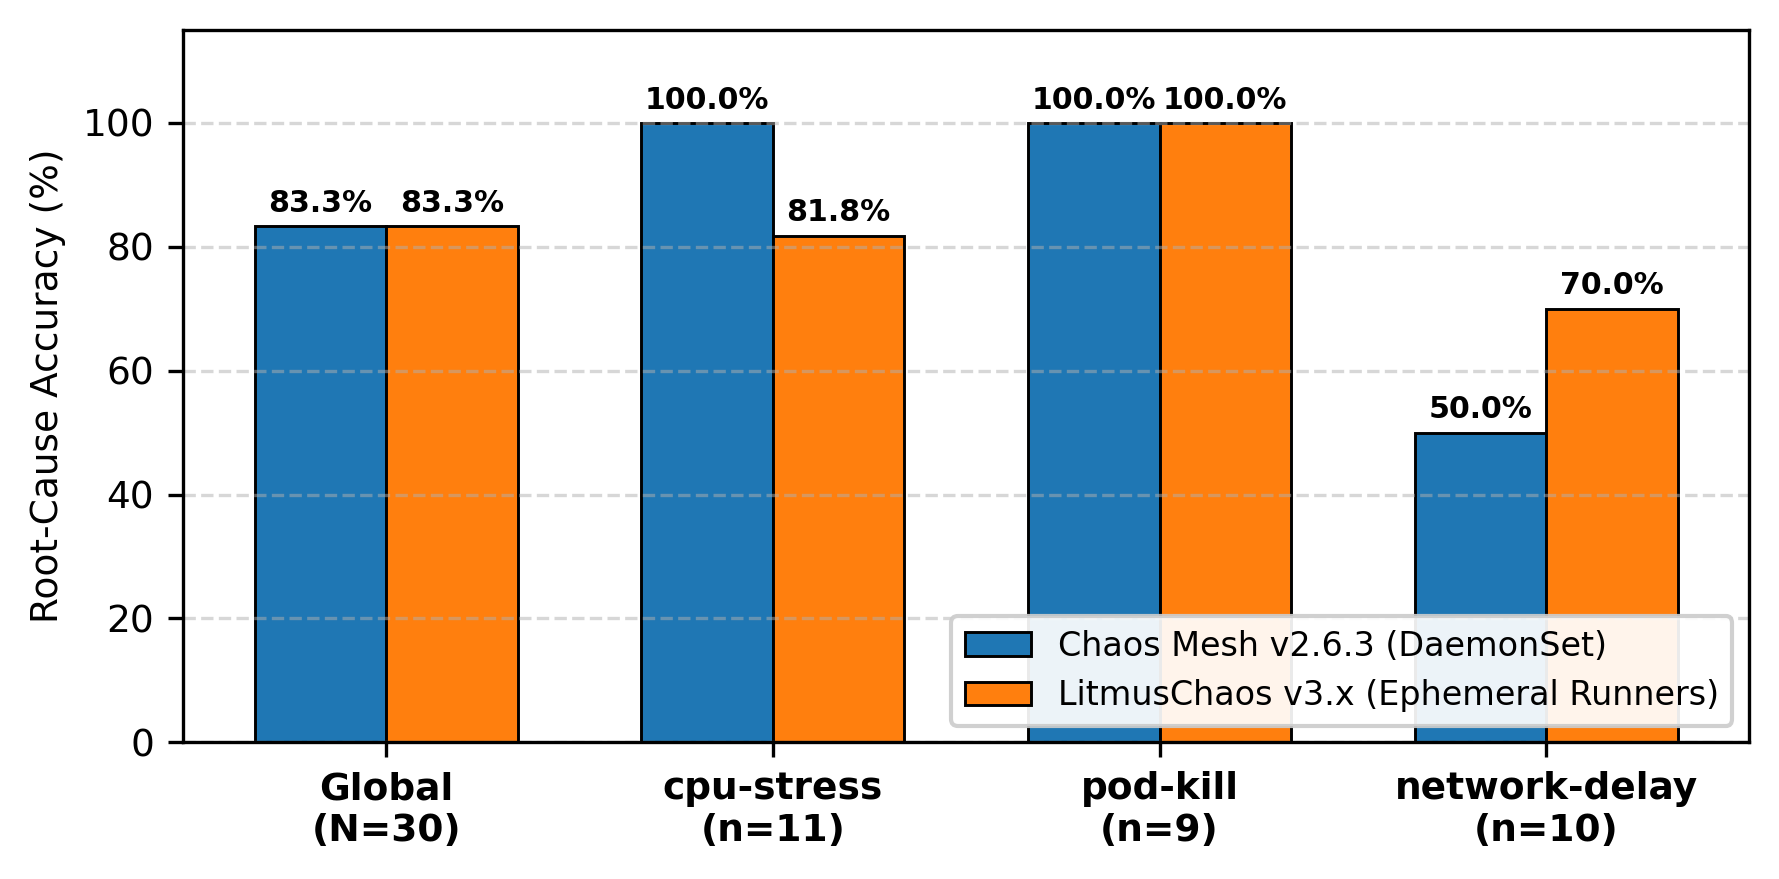
\includegraphics[width=0.96\columnwidth]{figures/fig_stratified_accuracy_cm_vs_lc.png}
\caption{Global and stratified root-cause diagnostic accuracy ($Acc$) comparing Chaos Mesh v2.6.3 and LitmusChaos v3.x over $N=30$ paired trials.}
\Description{Grouped bar chart showing identical 83.3 percent global accuracy across Chaos Mesh and LitmusChaos, with stratified percentages across cpu-stress, pod-kill, and network-delay.}
\label{fig:accuracy_cm_vs_lc}
\end{figure}

Analyzing the stratified diagnostic dynamics and latency distributions reveals three notable insights:
\begin{enumerate}
    \item \textbf{Mean Net Convergence Equivalence vs.\ Median Helper-Container Offset:} Across all $30$ trials, subtracting $\Delta T_{\text{actuate}}$ brought LitmusChaos's mean net diagnostic latency ($MTTDiag_{\text{net}} = 57.35 \pm 67.58\,\text{s}$) into close agreement with Chaos Mesh ($54.52 \pm 98.41\,\text{s}$). On resolved trials ($n=25$), LitmusChaos's median $MTTDiag_{\text{net}}$ was $42.17\,\text{s}$ (total $53.97\,\text{s}$) compared to $16.85\,\text{s}$ in Chaos Mesh ($W = 55.0$, $p = 7.51 \times 10^{-4}$), because after \texttt{go-runner} pod creation ($T_{\text{effect}}$), the helper container still requires $\sim 15\text{--}20\,\text{s}$ to initialize its internal experiment binary, inspect target container PIDs via the container runtime socket, and ramp up the stressor.
    \item \textbf{Complementary Stratum Performance:} Both platforms achieved $\mathbf{100.0\%}$ ($9/9$) accuracy on \texttt{pod-kill}. On \texttt{network-delay}, LitmusChaos resolved $\mathbf{7/10}$ ($70.0\%$, including all $3/3$ \texttt{shipping} trials via Loki-to-Tempo error correlation and $4/4$ \texttt{cart}/\texttt{currency} trials via Tempo exclusive self-time $T_{\text{self}} \in [1977.7, 3349.3]\,\text{ms}$) compared to $5/10$ ($50.0\%$) in Chaos Mesh, whereas Chaos Mesh resolved $\mathbf{11/11}$ ($100.0\%$) on \texttt{cpu-stress} compared to $9/11$ ($81.8\%$) in LitmusChaos (where $2$ trials experienced transient downstream \texttt{payment} trace spikes before \texttt{go-runner} CPU hogging reached full cgroup saturation).
    \item \textbf{Multimodal Detection Breakdown in LitmusChaos:} Among the $25$ successful LitmusChaos diagnoses, $10$ ($40\%$) converged via \texttt{PROMETHEUS\_\allowbreak METRIC\_\allowbreak SATURATION} ($\Delta_{\text{CPU}} \in [+383.8,\allowbreak +1203.9]\,\text{mCPU}$ and container restart counters), $6$ ($24\%$) via \texttt{LOKI\_\allowbreak TO\_\allowbreak TEMPO\_\allowbreak CORRELATION}, $4$ ($16\%$) via \texttt{LOKI\_\allowbreak LOG\_\allowbreak SIGNATURE} (\texttt{SIGTERM} capture), $4$ ($16\%$) via \texttt{TEMPO\_\allowbreak SELF\_\allowbreak TIME}, and $1$ ($4\%$) via \texttt{TEMPO\_\allowbreak TRACE\_\allowbreak ERROR}.
\end{enumerate}

\subsection{RQ04: Expressiveness of Native Steady-State Verification Probes}
Our experimental campaign also confirmed Hypothesis~$H_{1,4}$ regarding native verification capabilities. Whereas Chaos Mesh's native \texttt{StatusCheck} CRD is restricted to external HTTP status/latency polling—incapable of querying internal Prometheus cgroup metrics to isolate process-invisible \texttt{cpu-stress} saturation—LitmusChaos natively executed inline steady-state probes within the \texttt{ChaosEngine} lifecycle and exported structured \texttt{ChaosResult} verdicts (\texttt{probeSuccessPercentage = 100\%} when target deployment replica recovery invariants held at End-of-Test). By combining \texttt{promProbe} (PromQL threshold assertions) and \texttt{k8sProbe} (resource readiness invariants) in \texttt{Continuous} mode, LitmusChaos enables self-contained CI/CD resilience gating without external orchestration scripts.